\documentclass[]{article}
\usepackage{lmodern}
\usepackage{amssymb,amsmath}
\usepackage{ifxetex,ifluatex}
\usepackage{fixltx2e} % provides \textsubscript
\ifnum 0\ifxetex 1\fi\ifluatex 1\fi=0 % if pdftex
  \usepackage[T1]{fontenc}
  \usepackage[utf8]{inputenc}
\else % if luatex or xelatex
  \ifxetex
    \usepackage{mathspec}
    \usepackage{xltxtra,xunicode}
  \else
    \usepackage{fontspec}
  \fi
  \defaultfontfeatures{Mapping=tex-text,Scale=MatchLowercase}
  \newcommand{\euro}{€}
\fi
% use upquote if available, for straight quotes in verbatim environments
\IfFileExists{upquote.sty}{\usepackage{upquote}}{}
% use microtype if available
\IfFileExists{microtype.sty}{%
\usepackage{microtype}
\UseMicrotypeSet[protrusion]{basicmath} % disable protrusion for tt fonts
}{}
\usepackage[margin=1in]{geometry}
\usepackage{color}
\usepackage{fancyvrb}
\newcommand{\VerbBar}{|}
\newcommand{\VERB}{\Verb[commandchars=\\\{\}]}
\DefineVerbatimEnvironment{Highlighting}{Verbatim}{commandchars=\\\{\}}
% Add ',fontsize=\small' for more characters per line
\usepackage{framed}
\definecolor{shadecolor}{RGB}{248,248,248}
\newenvironment{Shaded}{\begin{snugshade}}{\end{snugshade}}
\newcommand{\KeywordTok}[1]{\textcolor[rgb]{0.13,0.29,0.53}{\textbf{{#1}}}}
\newcommand{\DataTypeTok}[1]{\textcolor[rgb]{0.13,0.29,0.53}{{#1}}}
\newcommand{\DecValTok}[1]{\textcolor[rgb]{0.00,0.00,0.81}{{#1}}}
\newcommand{\BaseNTok}[1]{\textcolor[rgb]{0.00,0.00,0.81}{{#1}}}
\newcommand{\FloatTok}[1]{\textcolor[rgb]{0.00,0.00,0.81}{{#1}}}
\newcommand{\CharTok}[1]{\textcolor[rgb]{0.31,0.60,0.02}{{#1}}}
\newcommand{\StringTok}[1]{\textcolor[rgb]{0.31,0.60,0.02}{{#1}}}
\newcommand{\CommentTok}[1]{\textcolor[rgb]{0.56,0.35,0.01}{\textit{{#1}}}}
\newcommand{\OtherTok}[1]{\textcolor[rgb]{0.56,0.35,0.01}{{#1}}}
\newcommand{\AlertTok}[1]{\textcolor[rgb]{0.94,0.16,0.16}{{#1}}}
\newcommand{\FunctionTok}[1]{\textcolor[rgb]{0.00,0.00,0.00}{{#1}}}
\newcommand{\RegionMarkerTok}[1]{{#1}}
\newcommand{\ErrorTok}[1]{\textbf{{#1}}}
\newcommand{\NormalTok}[1]{{#1}}
\usepackage{longtable,booktabs}
\usepackage{graphicx}
\makeatletter
\def\maxwidth{\ifdim\Gin@nat@width>\linewidth\linewidth\else\Gin@nat@width\fi}
\def\maxheight{\ifdim\Gin@nat@height>\textheight\textheight\else\Gin@nat@height\fi}
\makeatother
% Scale images if necessary, so that they will not overflow the page
% margins by default, and it is still possible to overwrite the defaults
% using explicit options in \includegraphics[width, height, ...]{}
\setkeys{Gin}{width=\maxwidth,height=\maxheight,keepaspectratio}
\ifxetex
  \usepackage[setpagesize=false, % page size defined by xetex
              unicode=false, % unicode breaks when used with xetex
              xetex]{hyperref}
\else
  \usepackage[unicode=true]{hyperref}
\fi
\hypersetup{breaklinks=true,
            bookmarks=true,
            pdfauthor={JcB},
            pdftitle={Date de naissance, âge et sexe},
            colorlinks=true,
            citecolor=blue,
            urlcolor=blue,
            linkcolor=magenta,
            pdfborder={0 0 0}}
\urlstyle{same}  % don't use monospace font for urls
\setlength{\parindent}{0pt}
\setlength{\parskip}{6pt plus 2pt minus 1pt}
\setlength{\emergencystretch}{3em}  % prevent overfull lines
\setcounter{secnumdepth}{5}

%%% Use protect on footnotes to avoid problems with footnotes in titles
\let\rmarkdownfootnote\footnote%
\def\footnote{\protect\rmarkdownfootnote}

%%% Change title format to be more compact
\usepackage{titling}
\setlength{\droptitle}{-2em}
  \title{Date de naissance, âge et sexe}
  \pretitle{\vspace{\droptitle}\centering\huge}
  \posttitle{\par}
  \author{JcB}
  \preauthor{\centering\large\emph}
  \postauthor{\par}
  \predate{\centering\large\emph}
  \postdate{\par}
  \date{31/10/2014}




\begin{document}

\maketitle


{
\hypersetup{linkcolor=black}
\setcounter{tocdepth}{2}
\tableofcontents
}
\section{Introduction}\label{introduction}

Ce document adapte les recommandations de la FEDORU
\footnote{Collecte et usages des RPU. Recommandations sur la production, les définitions, la qualité et l'exploitation des données des Résumés de Passage aux Urgences. FEDORU 2014 - V01-10/2014}.

La \textbf{date de naissance} du patient, attendue au format
``JJ/MM/AAAA'' au sein des RPU, est automatiquement croisée avec la date
d'entree aux urgences pour permetttre le calcul de l'âge. Les âges de
plus de $120$ ans sont considérés comme des valeurs aberrantes et sont
exclus de l'analyse. Il en va de même pour les âges négatifs.

Le \textbf{sexe} sont au format ``M/F/I''.

\subsection{Recommandations FEDORU
2014}\label{recommandations-fedoru-2014}

La FEDORU recommande l'harmonisation des analyses des données selon les
formats suivants:

\begin{itemize}
\item
  Age = date d'entrée - date de naissance
\item
  Critères d'exclusion: age négatif et age \textgreater{} 120 ans (43800
  jours)
\item
  nourissons \textless{} 28 jours
\item
  Tranches d'age pour les moins de 18 ans
\item
  \textless{} 28 jours
\item
  {[}28 jours à 1 an{[}
\item
  {[}1 an à 5 ans{[}
\item
  {[}5 ans à 10 ans{[}
\item
  {[}10 à 15 ans{[}
\item
  {[}15 ans à 18 ans{[}
\item
  Tranches d'age pour les adultes:
\item
  {[}18-30ans{[}
\item
  {[}30-45ans{[}
\item
  {[}45-65ans{[}
\item
  {[}65-75ans{[}
\item
  {[}75-85ans{[}
\item
  \begin{quote}
  85ans
  \end{quote}
\end{itemize}

ref: {[}Introduction à R{]} pp 68 pour définir les intervalles

\begin{Shaded}
\begin{Highlighting}[]
\NormalTok{ped_jours <-}\StringTok{ }\KeywordTok{c}\NormalTok{(}\DecValTok{1}\NormalTok{, }\DecValTok{28}\NormalTok{, }\KeywordTok{c}\NormalTok{(}\DecValTok{1}\NormalTok{, }\DecValTok{5}\NormalTok{, }\DecValTok{10}\NormalTok{, }\DecValTok{15}\NormalTok{, }\DecValTok{18}\NormalTok{) *}\StringTok{ }\DecValTok{365}\NormalTok{) }\CommentTok{# bornes pour la pédiatrie en jour}
\NormalTok{ped_jours}
\end{Highlighting}
\end{Shaded}

\begin{verbatim}
## [1]    1   28  365 1825 3650 5475 6570
\end{verbatim}

\begin{Shaded}
\begin{Highlighting}[]
\NormalTok{adultes_jours <-}\StringTok{ }\KeywordTok{c}\NormalTok{(}\DecValTok{18}\NormalTok{, }\DecValTok{30}\NormalTok{, }\DecValTok{45}\NormalTok{, }\DecValTok{65}\NormalTok{, }\DecValTok{75}\NormalTok{, }\DecValTok{85}\NormalTok{, }\DecValTok{120}\NormalTok{) *}\StringTok{ }\DecValTok{365}
\NormalTok{adultes_jours}
\end{Highlighting}
\end{Shaded}

\begin{verbatim}
## [1]  6570 10950 16425 23725 27375 31025 43800
\end{verbatim}

\begin{Shaded}
\begin{Highlighting}[]
\NormalTok{adultes_ans <-}\StringTok{ }\KeywordTok{c}\NormalTok{(}\DecValTok{18}\NormalTok{, }\DecValTok{30}\NormalTok{, }\DecValTok{45}\NormalTok{, }\DecValTok{65}\NormalTok{, }\DecValTok{75}\NormalTok{, }\DecValTok{85}\NormalTok{, }\DecValTok{120}\NormalTok{)}
\end{Highlighting}
\end{Shaded}

\begin{Shaded}
\begin{Highlighting}[]
\KeywordTok{library}\NormalTok{(lubridate)}
\KeywordTok{load}\NormalTok{(}\StringTok{"~/Documents/Resural/Stat Resural/RPU_2014/rpu2014d0112_c.Rda"}\NormalTok{)}
\NormalTok{dx <-}\StringTok{ }\NormalTok{d14}
\NormalTok{N <-}\StringTok{ }\KeywordTok{nrow}\NormalTok{(dx)}
\end{Highlighting}
\end{Shaded}

\subsection{Tranches d'age
pédiatriques:}\label{tranches-dage-pediatriques}

\begin{Shaded}
\begin{Highlighting}[]
\CommentTok{# age est un objet de type difftime exprimé en jours}
\NormalTok{age <-}\StringTok{ }\KeywordTok{as.Date}\NormalTok{(dx$ENTREE) -}\StringTok{ }\KeywordTok{as.Date}\NormalTok{(dx$NAISSANCE)}
\NormalTok{age <-}\StringTok{ }\KeywordTok{as.numeric}\NormalTok{(age)}

\CommentTok{# on retire les valeurs aberrantes: mois de 1 jour et plus de 120 ans}
\NormalTok{age <-}\StringTok{ }\NormalTok{age[age >}\StringTok{ }\DecValTok{1} \NormalTok{&}\StringTok{ }\NormalTok{age <=}\StringTok{ }\DecValTok{365}\NormalTok{*}\DecValTok{120}\NormalTok{]}
\NormalTok{age_an <-}\StringTok{ }\KeywordTok{round}\NormalTok{(age/}\DecValTok{365}\NormalTok{, }\DecValTok{0}\NormalTok{)}

\CommentTok{# nombre de valeurs aberrantes}
\NormalTok{N -}\StringTok{ }\KeywordTok{length}\NormalTok{(age)}
\end{Highlighting}
\end{Shaded}

\begin{verbatim}
## [1] 36
\end{verbatim}

\begin{Shaded}
\begin{Highlighting}[]
\CommentTok{# histogramme de age}
\KeywordTok{hist}\NormalTok{(age, }\DataTypeTok{main=}\StringTok{"Histogramme des ages en jours"}\NormalTok{, }\DataTypeTok{xlab =} \StringTok{"Age (en jours)"}\NormalTok{, }\DataTypeTok{ylab =} \StringTok{"Fréquence"}\NormalTok{)}
\end{Highlighting}
\end{Shaded}

\begin{figure}[htbp]
\centering
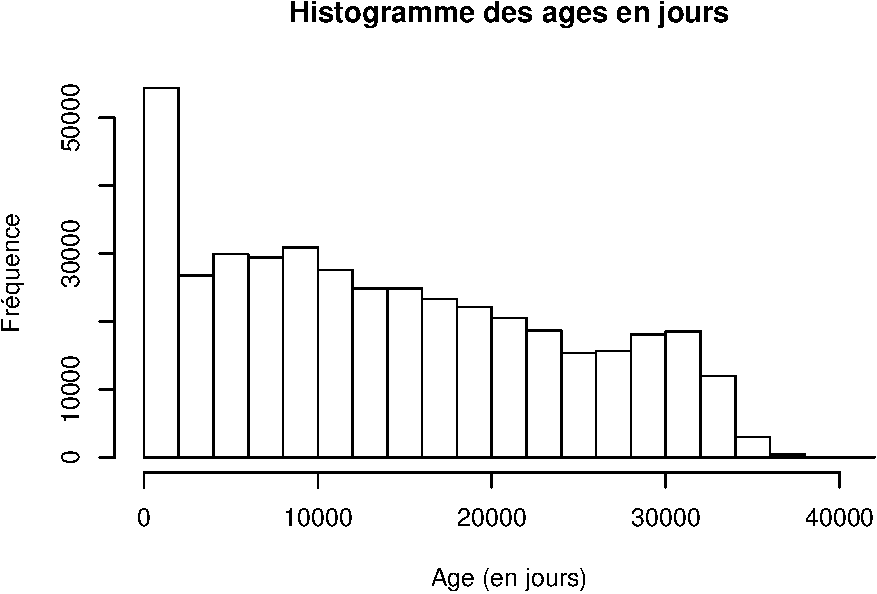
\includegraphics{age_files/figure-latex/ped-1.pdf}
\end{figure}

\begin{Shaded}
\begin{Highlighting}[]
\CommentTok{# les moins de 1 an = age1}
\NormalTok{age1 <-}\StringTok{ }\NormalTok{age[age <}\StringTok{ }\DecValTok{366}\NormalTok{]}
\NormalTok{n_age1 <-}\StringTok{ }\KeywordTok{length}\NormalTok{(age1) }\CommentTok{# nombre de moins d'un an}
\NormalTok{p_age1 <-}\StringTok{ }\KeywordTok{round}\NormalTok{(}\KeywordTok{length}\NormalTok{(age1)*}\DecValTok{100}\NormalTok{/N, }\DecValTok{2}\NormalTok{) }\CommentTok{# proportion de moins de 1 an}
\KeywordTok{hist}\NormalTok{(age1, }\DataTypeTok{main =} \StringTok{"Histogramme des moins de 1 an"}\NormalTok{, }\DataTypeTok{xlab =} \StringTok{"Age en jours"}\NormalTok{, }\DataTypeTok{ylab =} \StringTok{"Fréquence"}\NormalTok{)}
\KeywordTok{abline}\NormalTok{(}\DataTypeTok{v=}\DecValTok{28}\NormalTok{, }\DataTypeTok{lty=}\DecValTok{2}\NormalTok{, }\DataTypeTok{col=}\StringTok{"red"}\NormalTok{) }\CommentTok{# limite nourissons}
\end{Highlighting}
\end{Shaded}

\begin{figure}[htbp]
\centering
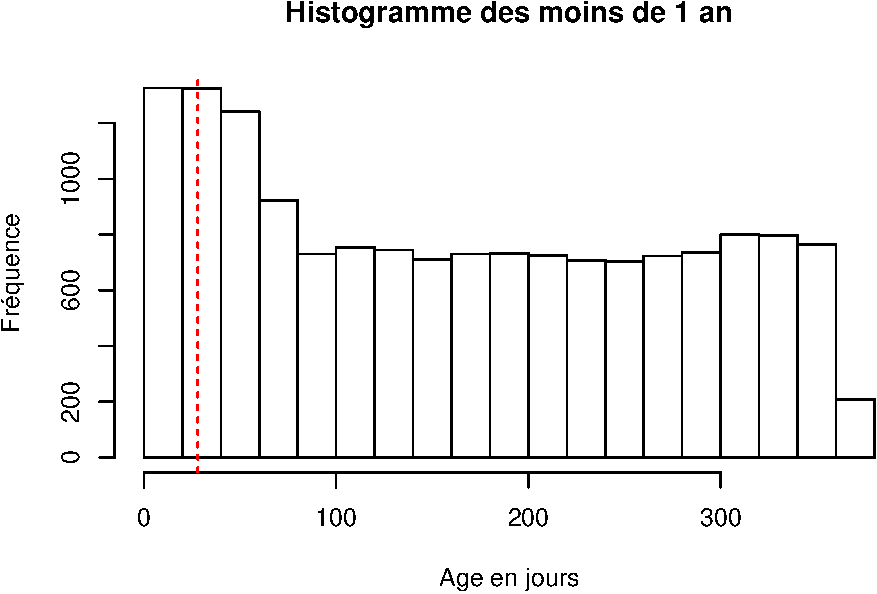
\includegraphics{age_files/figure-latex/ped-2.pdf}
\end{figure}

\begin{Shaded}
\begin{Highlighting}[]
\CommentTok{# nourissons age < 28 jours}
\NormalTok{nour <-}\StringTok{ }\NormalTok{age[age <}\StringTok{ }\DecValTok{28}\NormalTok{]}
\NormalTok{n_nour <-}\StringTok{ }\KeywordTok{length}\NormalTok{(nour)}

\CommentTok{# classes FEDORU pour la pédiatrie. La borne inférieure est incluse (include.lowest) et la borne sup est exclue (right = FALSE)}
\NormalTok{lab <-}\StringTok{ }\KeywordTok{c}\NormalTok{(}\StringTok{"<28j"}\NormalTok{, }\StringTok{"28j-1an["}\NormalTok{, }\StringTok{"1-5ans["}\NormalTok{, }\StringTok{"5-10ans["}\NormalTok{, }\StringTok{"10-15ans["}\NormalTok{, }\StringTok{"15-18ans["}\NormalTok{)}
\NormalTok{ped <-}\StringTok{ }\KeywordTok{cut}\NormalTok{(age, ped_jours, }\DataTypeTok{include.lowest =} \OtherTok{TRUE}\NormalTok{, }\DataTypeTok{right =} \OtherTok{FALSE}\NormalTok{, }\DataTypeTok{labels =} \NormalTok{lab)}

\KeywordTok{table}\NormalTok{(ped)}
\end{Highlighting}
\end{Shaded}

\begin{verbatim}
## ped
##      <28j  28j-1an[   1-5ans[  5-10ans[ 10-15ans[ 15-18ans[ 
##      1791     13554     36287     24738     27012     15819
\end{verbatim}

\begin{Shaded}
\begin{Highlighting}[]
\KeywordTok{barplot}\NormalTok{(}\KeywordTok{table}\NormalTok{(ped), }\DataTypeTok{main =} \StringTok{"Pédiatrie"}\NormalTok{)}
\end{Highlighting}
\end{Shaded}

\begin{figure}[htbp]
\centering
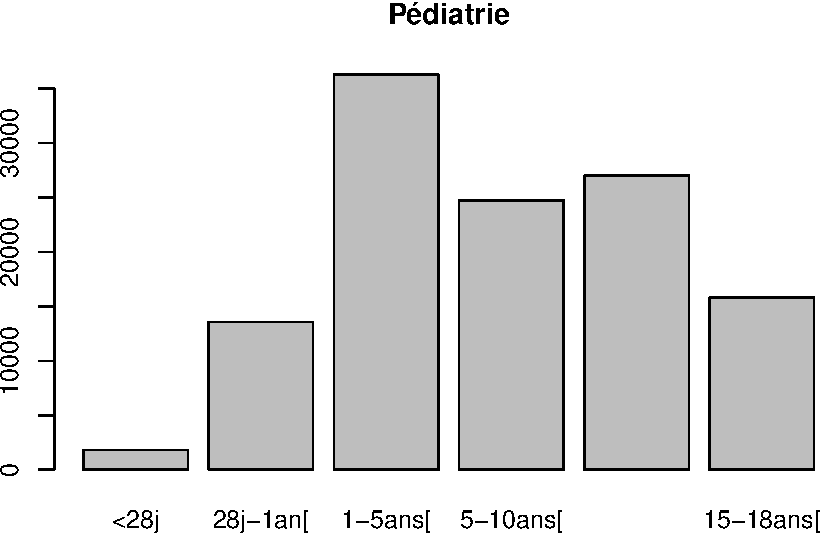
\includegraphics{age_files/figure-latex/ped-3.pdf}
\end{figure}

\subsection{Tranches d'age adultes}\label{tranches-dage-adultes}

\begin{Shaded}
\begin{Highlighting}[]
\NormalTok{lab_adultes <-}\StringTok{ }\KeywordTok{c}\NormalTok{(}\StringTok{"18-30ans"}\NormalTok{, }\StringTok{"30-45ans"}\NormalTok{, }\StringTok{"45-65ans"}\NormalTok{, }\StringTok{"65-75ans"}\NormalTok{, }\StringTok{"75-85ans"}\NormalTok{, }\StringTok{">85ans"}\NormalTok{)}
\NormalTok{adultes <-}\StringTok{ }\KeywordTok{cut}\NormalTok{(age, adultes_jours, }\DataTypeTok{include.lowest =} \OtherTok{TRUE}\NormalTok{, }\DataTypeTok{right =} \OtherTok{FALSE}\NormalTok{, }\DataTypeTok{labels =} \NormalTok{lab_adultes)}
\NormalTok{adultes_rpu <-}\StringTok{ }\KeywordTok{table}\NormalTok{(adultes)}

\KeywordTok{barplot}\NormalTok{(adultes_rpu, }\DataTypeTok{main=}\StringTok{"RPU adultes en fonction des classes d'âge de la FEDORU"}\NormalTok{)}
\end{Highlighting}
\end{Shaded}

\begin{figure}[htbp]
\centering
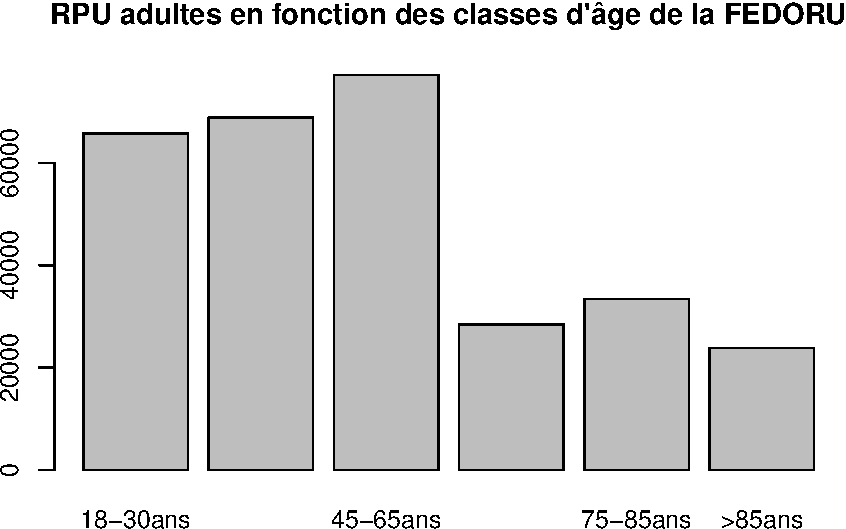
\includegraphics{age_files/figure-latex/adultes-1.pdf}
\end{figure}

\begin{Shaded}
\begin{Highlighting}[]
\CommentTok{# idel en %}
\KeywordTok{barplot}\NormalTok{(adultes_rpu*}\DecValTok{100}\NormalTok{/N, }\DataTypeTok{main=}\StringTok{"RPU adultes en fonction des classes d'âge de la FEDORU"}\NormalTok{)}
\end{Highlighting}
\end{Shaded}

\begin{figure}[htbp]
\centering
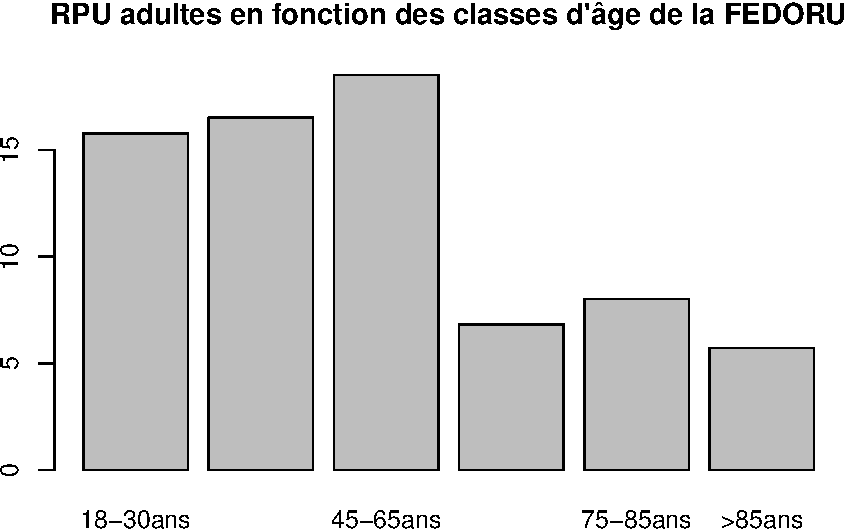
\includegraphics{age_files/figure-latex/adultes-2.pdf}
\end{figure}

\section{Sexe (RPU)}\label{sexe-rpu}

\begin{Shaded}
\begin{Highlighting}[]
\NormalTok{sexe <-}\StringTok{ }\KeywordTok{table}\NormalTok{(dx$SEXE)}
\NormalTok{h_rpu <-}\StringTok{ }\NormalTok{sexe[}\DecValTok{2}\NormalTok{]}
\NormalTok{f_rpu <-}\StringTok{ }\NormalTok{sexe[}\DecValTok{1}\NormalTok{]}
\NormalTok{sex_ratio <-}\StringTok{ }\KeywordTok{round}\NormalTok{(h_rpu/f_rpu, }\DecValTok{2}\NormalTok{)}
\NormalTok{r_masculinite <-}\StringTok{ }\KeywordTok{round}\NormalTok{(h_rpu/(h_rpu +}\StringTok{ }\NormalTok{f_rpu), }\DecValTok{2}\NormalTok{)}
\KeywordTok{pie}\NormalTok{(sexe, }\DataTypeTok{col=}\KeywordTok{c}\NormalTok{(}\StringTok{"red"}\NormalTok{, }\StringTok{"yellow"}\NormalTok{), }\DataTypeTok{labels=}\KeywordTok{c}\NormalTok{(}\StringTok{"Femmes"}\NormalTok{,}\StringTok{"Hommes"}\NormalTok{))}
\end{Highlighting}
\end{Shaded}

\begin{figure}[htbp]
\centering
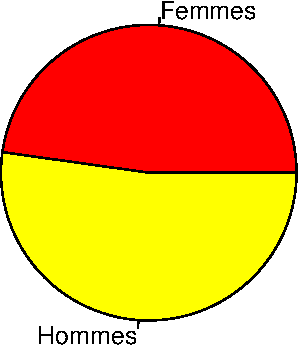
\includegraphics{age_files/figure-latex/sexe-1.pdf}
\end{figure}

\begin{Shaded}
\begin{Highlighting}[]
\CommentTok{# calcul du vecteur sex-ratio: pour chaque tranche d'age de 1 an, on calcule de sr. On ne retient que les lignes 1 (femmes) et 2 (hommes). Le résultat (a) est une matrice à 2 lignes et une centaine de colonnes:}
\NormalTok{a <-}\StringTok{ }\KeywordTok{tapply}\NormalTok{(}\KeywordTok{as.Date}\NormalTok{(dx$ENTREE), }\KeywordTok{list}\NormalTok{(dx$SEXE, dx$AGE), length)}
\NormalTok{a <-}\StringTok{ }\NormalTok{a[}\DecValTok{1}\NormalTok{:}\DecValTok{2}\NormalTok{,]}
\NormalTok{sr_age_rpu <-}\StringTok{ }\NormalTok{a[}\DecValTok{2}\NormalTok{,]/a[}\DecValTok{1}\NormalTok{,]}
\KeywordTok{plot}\NormalTok{(sr_age_rpu, }\DataTypeTok{type=}\StringTok{"l"}\NormalTok{, }\DataTypeTok{main=}\StringTok{"Evolution du sexe-ratio en fonction de l'âge"}\NormalTok{, }\DataTypeTok{ylab=}\StringTok{"Sexe-ratio"}\NormalTok{, }\DataTypeTok{xlab=}\StringTok{"Age (années)"}\NormalTok{, }\DataTypeTok{lwd=}\DecValTok{3}\NormalTok{, }\DataTypeTok{col=}\StringTok{"red"}\NormalTok{)}
\KeywordTok{abline}\NormalTok{(}\DataTypeTok{h=}\DecValTok{1}\NormalTok{, }\DataTypeTok{lty=}\DecValTok{2}\NormalTok{)}
\end{Highlighting}
\end{Shaded}

\begin{figure}[htbp]
\centering
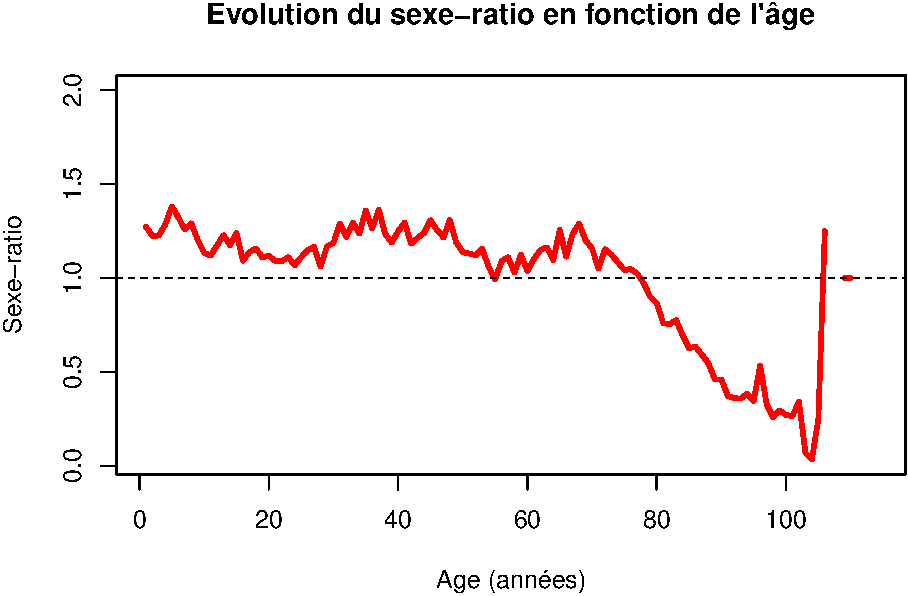
\includegraphics{age_files/figure-latex/sexe-2.pdf}
\end{figure}

\begin{itemize}
\itemsep1pt\parskip0pt\parsep0pt
\item
  nombre d'hommes 217 617
\item
  nombre de femmes 199 110
\item
  sex-ratio 1.1
\item
  rapport de masculinité 0.52
\end{itemize}

\section{Résumé RPU}\label{resume-rpu}

\begin{longtable}[c]{@{}lll@{}}
\toprule\addlinespace
Variables & intitulé en clair & valeur
\\\addlinespace
\midrule\endhead
N & nombre total de RPU & 416 733
\\\addlinespace
age & ages des consultants en jours de 1 jour à 120 ans & \emph{vecteur}
\\\addlinespace
age\_an & age des consultants en années & \emph{vecteur}
\\\addlinespace
sex\_ratio & sexe-ratio & 1.1
\\\addlinespace
r\_masculinite & taux de masculinité = nb hommes / (hommes + femmes) &
0.52
\\\addlinespace
sr\_age\_rpu & vecteur des sex-ratio & \emph{vecteur}
\\\addlinespace
h\_rpu & nombre d'hommes & 217 617
\\\addlinespace
f\_rpu & nombre de femmes & 199 110
\\\addlinespace
n\_age1 & nombre de moins d'un an & 15 385
\\\addlinespace
p\_age1 & proportion de moins d'un an & 3.7
\\\addlinespace
n\_nour & nombre de nourrisons (\textless{} 28 jours) & 1 791
\\\addlinespace
adultes & vecteur ages \textgreater{} 18 ans selon FEDORU &
\emph{vecteur}
\\\addlinespace
adultes\_rpu & table(adultes) & \emph{table}
\\\addlinespace
adultes\_jours & bornes intervalles adulte en jours & \emph{vecteur}
\\\addlinespace
adultes\_ans & bornes intervalles adulte en années & \emph{vecteur}
\\\addlinespace
lab\_adultes & vecteur de labels pour tranches âge &
\\\addlinespace
ped\_jours & bornes intervalles ped. en jours & \emph{vecteur}
\\\addlinespace
ped & vecteur des tranches d'âge pediatriques & \emph{vecteur}
\\\addlinespace
lab & vecteur de labels pour table(ped) &
\\\addlinespace
\bottomrule
\end{longtable}

\section{Population d'Alsace}\label{population-dalsace}

La comparaison de la pyramide des ages de la;patientèle des urgences à
celle de la population de la même,zone géographique est également
informative. Ele nécessite pour cela de connaître la structure de la
population en Alsace. Pour cela on utilise des données de l'INSEE.

source:
\url{http://www.insee.fr/fr/ppp/bases-de-donnees/donnees-detaillees/rp2011/tab-detailles/td-population-11/BTT_TD_POP1B_2011.zip}

Ce fichier recense pour chaque commune de France la population par
\textbf{sexe} et \textbf{tranches d'ages de 1 an} de 0 à 100 ans. La
version \emph{POP1B}2011\_ est le fichier légal pour 2014.

Le fichier dézippé fait 220 Mo. Il est stocké à l'adresse suivante:

Après plusieurs essais, la meilleure méthode pour lire ce fichier est
d'utiliser \textbf{read.csv2}, le séparateur étant le
\textbf{point-virgule}. L'utilisation de \emph{encoding} est à procrire
car cela crée des ficheiers corrompus. L'inconvénient de la méthode est
de produire un codage anormal des caractères accentués qu'il faut
corriger:

\begin{longtable}[c]{@{}ll@{}}
\toprule\addlinespace
expression & symbole
\\\addlinespace
\midrule\endhead
\texttt{\textbackslash{}xe8} & è
\\\addlinespace
\texttt{\textbackslash{}xe9} & é
\\\addlinespace
\bottomrule
\end{longtable}

Les instructions qui suivent décrivent la procédure pour lire ce
ficchier et en extraire les données propres à l'Alsace. Les fichiers
suivant sont créés et peuvent être chargés directement pour exploiter
les données locales:

\begin{longtable}[c]{@{}ll@{}}
\toprule\addlinespace
fichier & Données
\\\addlinespace
\midrule\endhead
pop\_france\_2014.Rda & ensemble de la population française
\\\addlinespace
pop\_als\_2014.Rda & ensemble de la population alsacienne
\\\addlinespace
pop67\_2014.Rda & ensemble de la population du Bas-Rhin
\\\addlinespace
pop68\_2014.Rda & ensemble de la population du Haut-Rhin
\\\addlinespace
\bottomrule
\end{longtable}

\begin{verbatim}
file <- "/home/jcb/Documents/Resural/Stat Resural/population_alsace/BTT_TD_POP1B_2011.txt"
pop <- read.csv2(file)

# remplacer les caractères anormaux
pop$LIBGEO <- as.character(pop$LIBGEO)      # transforme le fateur en caractères
pop$LIBGEO <- gsub("\xe8","è", pop$LIBGEO)  # remplacement des caractères anormaux
pop$LIBGEO <- gsub("\xe9","é", pop$LIBGEO)

save(pop, file = "pop_france_2014.Rda")     # toute la France

names(pop)

# on extrait les populations d'Alsace

# population du 67. On supprime les levels exédentaires
pop67_2014 <- pop[substr(pop$CODGEO, 1, 2) == 67,]
pop67_2014$LIBGEO <- factor(pop67_2014$LIBGEO)
pop67_2014$CODGEO <- factor(pop67_2014$CODGEO)

# population du 68. On supprime les levels exédentaires
pop68_2014 <- pop[substr(pop$CODGEO, 1, 2) == 68,]
pop68_2014$LIBGEO <- factor(pop68_2014$LIBGEO)
pop68_2014$CODGEO <- factor(pop68_2014$CODGEO)

# population de la région Alsace
pop_als_2014 <- pop[substr(pop$CODGEO, 1, 2) == 67 | substr(pop$CODGEO, 1, 2) == 68,]
pop_als_2014$LIBGEO <- factor(pop_als_2014$LIBGEO)
pop_als_2014$CODGEO <- factor(pop_als_2014$CODGEO)

# Sauvegarde des données
save(pop_als_2014, file="pop_als_2014.Rda")
save(pop67_2014, file="pop67_2014.Rda")
save(pop68_2014, file="pop68_2014.Rda")

# Chargement des données
load("pop68_2014.Rda")
load("pop67_2014.Rda")
load("pop_als_2014.Rda")
\end{verbatim}

\subsection{Population alsacienne:}\label{population-alsacienne}

\begin{Shaded}
\begin{Highlighting}[]
\NormalTok{path <-}\StringTok{ "../"}
\KeywordTok{load}\NormalTok{(}\KeywordTok{paste0}\NormalTok{(path, }\StringTok{"pop68_2014.Rda"}\NormalTok{))}
\KeywordTok{load}\NormalTok{(}\KeywordTok{paste0}\NormalTok{(path, }\StringTok{"pop67_2014.Rda"}\NormalTok{))}
\KeywordTok{load}\NormalTok{(}\KeywordTok{paste0}\NormalTok{(path, }\StringTok{"pop_als_2014.Rda"}\NormalTok{))}

\NormalTok{n67_2014 <-}\StringTok{ }\KeywordTok{sum}\NormalTok{(pop67_2014$NB)}
\NormalTok{n68_2014 <-}\StringTok{ }\KeywordTok{sum}\NormalTok{(pop68_2014$NB)}
\NormalTok{nAls_2014 <-}\StringTok{ }\KeywordTok{sum}\NormalTok{(pop_als_2014$NB)}

\CommentTok{# pyramide des ages en Alsace en 2014: vecteur de 101 lignes. Chaque ligne correspond au total de la population pour la tranche d'age (tous sexes confondus.)}
\NormalTok{p_ages_als_2014 <-}\StringTok{ }\KeywordTok{tapply}\NormalTok{(pop_als_2014$NB, pop_als_2014$AGED100, sum)}

\CommentTok{# représentation graphique de la pyramide des ages avec en surimpression la pyramide des ages des RPU (ligne verte), tracée à partir du vecteur des ages en année (age_an). Le vecteur est transformé en table à partir de laquelle on détermine les valeurs de x et y pour dessinner la courbe.}
\KeywordTok{barplot}\NormalTok{(p_ages_als_2014, }\DataTypeTok{horiz=}\OtherTok{TRUE}\NormalTok{, }\DataTypeTok{las =} \DecValTok{1}\NormalTok{, }\DataTypeTok{main=}\StringTok{"Pramides des ages en Alsace (2014)"}\NormalTok{, }\DataTypeTok{ylab=}\StringTok{"Age (années)"}\NormalTok{, }\DataTypeTok{xlab=}\StringTok{"Fréquence"}\NormalTok{)}
\NormalTok{a <-}\StringTok{ }\KeywordTok{table}\NormalTok{(}\KeywordTok{as.factor}\NormalTok{(age_an))}
\NormalTok{x <-}\StringTok{ }\KeywordTok{as.numeric}\NormalTok{(a)}
\NormalTok{y <-}\StringTok{ }\KeywordTok{as.numeric}\NormalTok{(}\KeywordTok{names}\NormalTok{(a))}
\KeywordTok{lines}\NormalTok{(x,y, }\DataTypeTok{col =} \StringTok{"green"}\NormalTok{, }\DataTypeTok{lwd =} \DecValTok{3}\NormalTok{)}
\KeywordTok{legend}\NormalTok{(}\StringTok{"topright"}\NormalTok{, }\DataTypeTok{legend =} \StringTok{"RPU 2014"}\NormalTok{, }\DataTypeTok{col =} \StringTok{"green"}\NormalTok{, }\DataTypeTok{lwd =} \DecValTok{3}\NormalTok{, }\DataTypeTok{bty =} \StringTok{"n"}\NormalTok{)}
\end{Highlighting}
\end{Shaded}

\begin{figure}[htbp]
\centering
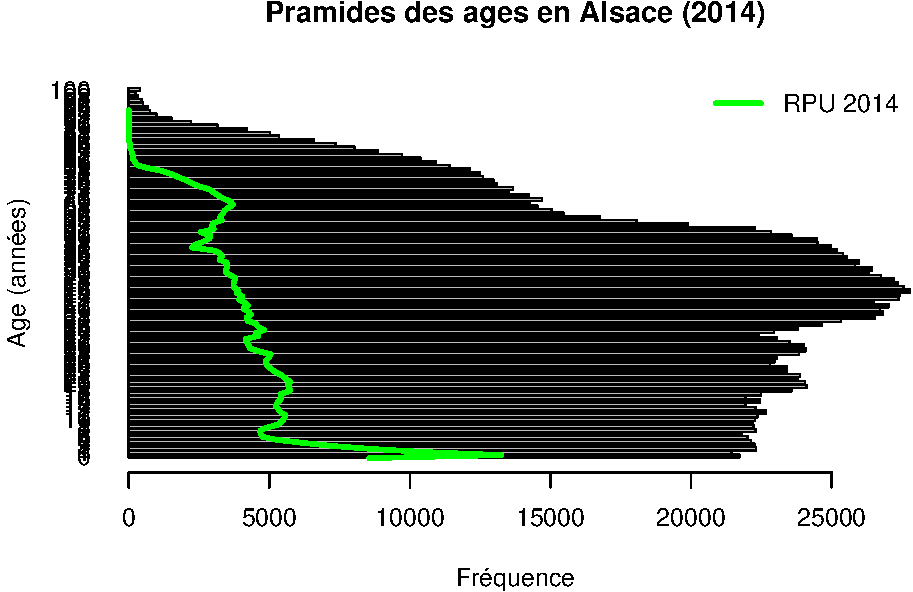
\includegraphics{age_files/figure-latex/pop_als-1.pdf}
\end{figure}

\begin{Shaded}
\begin{Highlighting}[]
\CommentTok{# Même représentation mais cette fois on utilise des pourcentages. Pour la pop alsacienne, l'effectif de chaque tranche est divisé par le nombre total d'habitants. Pour les RPU, l'effectif est divisé par le nombre total de RPU.}
\KeywordTok{barplot}\NormalTok{(p_ages_als_2014/nAls_2014, }\DataTypeTok{horiz=}\OtherTok{TRUE}\NormalTok{, }\DataTypeTok{las =} \DecValTok{1}\NormalTok{, }\DataTypeTok{main=}\StringTok{"Pramides des ages en Alsace (2014)"}\NormalTok{, }\DataTypeTok{ylab=}\StringTok{"Age (années)"}\NormalTok{, }\DataTypeTok{xlab=}\StringTok{"% de la population"}\NormalTok{)}
\NormalTok{a <-}\StringTok{ }\KeywordTok{table}\NormalTok{(}\KeywordTok{as.factor}\NormalTok{(age_an))}
\NormalTok{a <-}\StringTok{ }\NormalTok{a/N}
\NormalTok{x <-}\StringTok{ }\KeywordTok{as.numeric}\NormalTok{(a)}
\NormalTok{y <-}\StringTok{ }\KeywordTok{as.numeric}\NormalTok{(}\KeywordTok{names}\NormalTok{(a))}
\KeywordTok{lines}\NormalTok{(x,y, }\DataTypeTok{col =} \StringTok{"green"}\NormalTok{, }\DataTypeTok{lwd =} \DecValTok{3}\NormalTok{)}
\KeywordTok{legend}\NormalTok{(}\StringTok{"topright"}\NormalTok{, }\DataTypeTok{legend =} \StringTok{"RPU 2014"}\NormalTok{, }\DataTypeTok{col =} \StringTok{"green"}\NormalTok{, }\DataTypeTok{lwd =} \DecValTok{3}\NormalTok{, }\DataTypeTok{bty =} \StringTok{"n"}\NormalTok{)}
\end{Highlighting}
\end{Shaded}

\begin{figure}[htbp]
\centering
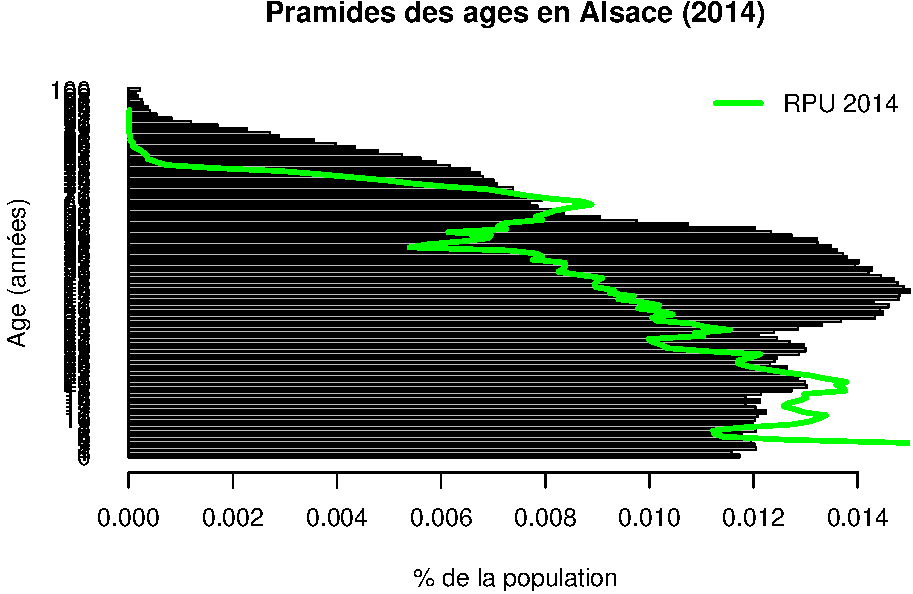
\includegraphics{age_files/figure-latex/pop_als-2.pdf}
\end{figure}

\begin{Shaded}
\begin{Highlighting}[]
\CommentTok{# calcul sur les sexes}
\NormalTok{sx <-}\StringTok{ }\KeywordTok{tapply}\NormalTok{(pop_als_2014$NB, pop_als_2014$SEXE, sum)}
\NormalTok{nh_als <-}\StringTok{ }\KeywordTok{as.numeric}\NormalTok{(sx[}\DecValTok{1}\NormalTok{])}
\NormalTok{nf_als <-}\StringTok{ }\KeywordTok{as.numeric}\NormalTok{(sx[}\DecValTok{2}\NormalTok{])}
\NormalTok{sexR_als <-}\StringTok{ }\NormalTok{nh_als/nf_als}
\NormalTok{masc_als <-}\StringTok{ }\NormalTok{nh_als/(nh_als+nf_als)}

\CommentTok{# sex ratio par tranche d'age. On utilise tappy en lui passant une liste de deux séparateur, le sexe et la tranche d'age. On récupère une matrice de 2 lignes (hommes, femmes) et 101 colonnes (les tranches d'age). La division des deux lignes renvoie le sex-ratio par tranche d'age de 1 an.}
\NormalTok{a <-}\StringTok{ }\KeywordTok{tapply}\NormalTok{(pop_als_2014$NB, }\KeywordTok{list}\NormalTok{(pop_als_2014$SEXE, pop_als_2014$AGED100), sum)}
\NormalTok{sr_age <-}\StringTok{ }\NormalTok{a[}\DecValTok{1}\NormalTok{,]/a[}\DecValTok{2}\NormalTok{,]}
\KeywordTok{plot}\NormalTok{(sr_age, }\DataTypeTok{type=}\StringTok{"l"}\NormalTok{, }\DataTypeTok{main=}\StringTok{"Evolution du sexe-ratio en fonction de l'âge"}\NormalTok{, }\DataTypeTok{ylab=}\StringTok{"Sexe-ratio"}\NormalTok{, }\DataTypeTok{xlab=}\StringTok{"Age (années)"}\NormalTok{, }\DataTypeTok{lwd=}\DecValTok{3}\NormalTok{, }\DataTypeTok{col=}\StringTok{"blue"}\NormalTok{)}
\KeywordTok{abline}\NormalTok{(}\DataTypeTok{h=}\DecValTok{1}\NormalTok{, }\DataTypeTok{lty=}\DecValTok{2}\NormalTok{)}
\end{Highlighting}
\end{Shaded}

\begin{figure}[htbp]
\centering
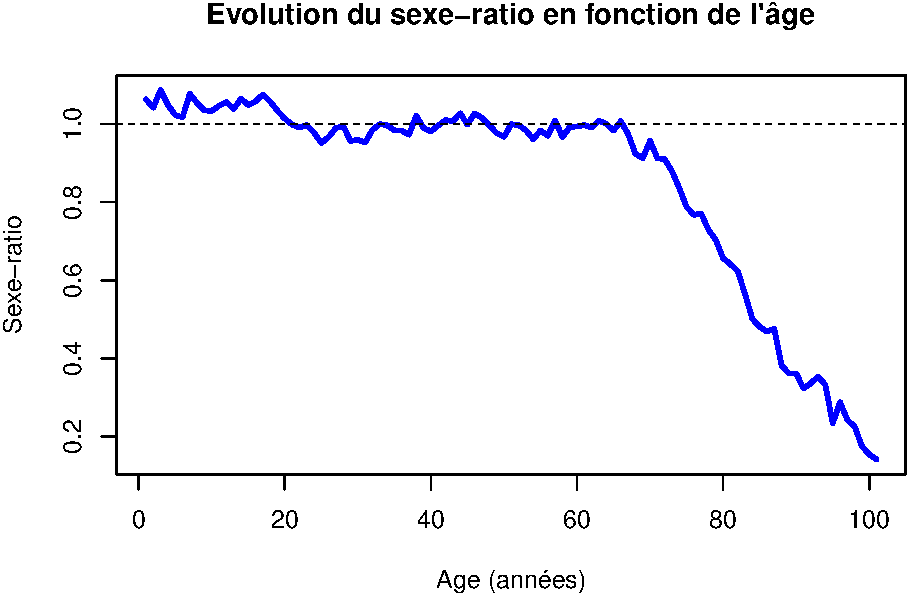
\includegraphics{age_files/figure-latex/pop_als-3.pdf}
\end{figure}

\begin{Shaded}
\begin{Highlighting}[]
\CommentTok{# Répartition de la population alsacienne en fonction des classes d'age de la Fedoru:}
\NormalTok{adultes_als <-}\StringTok{ }\KeywordTok{array}\NormalTok{()}
\NormalTok{adultes_als[}\DecValTok{1}\NormalTok{] <-}\StringTok{ }\KeywordTok{sum}\NormalTok{(p_ages_als_2014[}\DecValTok{18}\NormalTok{:}\DecValTok{29}\NormalTok{])}
\NormalTok{adultes_als[}\DecValTok{2}\NormalTok{] <-}\StringTok{ }\KeywordTok{sum}\NormalTok{(p_ages_als_2014[}\DecValTok{30}\NormalTok{:}\DecValTok{44}\NormalTok{])}
\NormalTok{adultes_als[}\DecValTok{3}\NormalTok{] <-}\StringTok{ }\KeywordTok{sum}\NormalTok{(p_ages_als_2014[}\DecValTok{45}\NormalTok{:}\DecValTok{64}\NormalTok{])}
\NormalTok{adultes_als[}\DecValTok{4}\NormalTok{] <-}\StringTok{ }\KeywordTok{sum}\NormalTok{(p_ages_als_2014[}\DecValTok{65}\NormalTok{:}\DecValTok{74}\NormalTok{])}
\NormalTok{adultes_als[}\DecValTok{5}\NormalTok{] <-}\StringTok{ }\KeywordTok{sum}\NormalTok{(p_ages_als_2014[}\DecValTok{75}\NormalTok{:}\DecValTok{84}\NormalTok{])}
\NormalTok{adultes_als[}\DecValTok{6}\NormalTok{] <-}\StringTok{ }\KeywordTok{sum}\NormalTok{(p_ages_als_2014[}\DecValTok{85}\NormalTok{:}\DecValTok{101}\NormalTok{])}
\KeywordTok{names}\NormalTok{(adultes_als) <-}\StringTok{ }\NormalTok{lab_adultes}
\NormalTok{adultes_als}
\end{Highlighting}
\end{Shaded}

\begin{verbatim}
## 18-30ans 30-45ans 45-65ans 65-75ans 75-85ans   >85ans 
##   281385   374784   507286   150229   114559    47760
\end{verbatim}

\begin{Shaded}
\begin{Highlighting}[]
\KeywordTok{barplot}\NormalTok{(adultes_als, }\DataTypeTok{main=}\StringTok{"Répartition de la population alsacienne adulte}\CharTok{\textbackslash{}n}\StringTok{ en fonction des classes d'âge de la Fedoru"}\NormalTok{)}
\end{Highlighting}
\end{Shaded}

\begin{figure}[htbp]
\centering
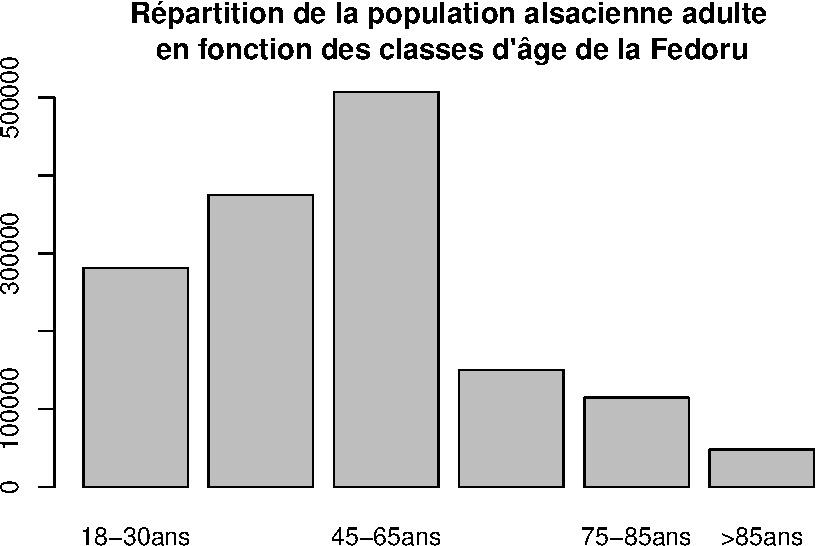
\includegraphics{age_files/figure-latex/pop_als-4.pdf}
\end{figure}

\begin{Shaded}
\begin{Highlighting}[]
\CommentTok{# en % de la population}
\KeywordTok{barplot}\NormalTok{(adultes_als*}\DecValTok{100}\NormalTok{/n67_2014, }\DataTypeTok{main=}\StringTok{"Répartition de la population alsacienne adulte}\CharTok{\textbackslash{}n}\StringTok{ en fonction des classes d'âge de la Fedoru"}\NormalTok{, }\DataTypeTok{las=}\DecValTok{1}\NormalTok{, }\DataTypeTok{ylab=}\StringTok{"% de la population"}\NormalTok{)}
\end{Highlighting}
\end{Shaded}

\begin{figure}[htbp]
\centering
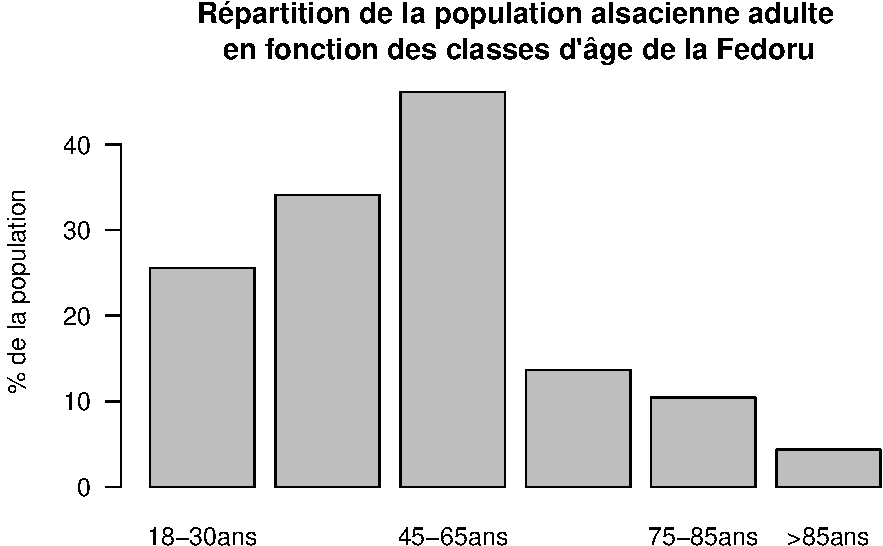
\includegraphics{age_files/figure-latex/pop_als-5.pdf}
\end{figure}

Variables crées:

\begin{itemize}
\itemsep1pt\parskip0pt\parsep0pt
\item
  n67\_2014: population totale du Bas-Rhin en 2014
\item
  n68\_2014: population totale du Haut-Rhin en 2014
\item
  nAls\_2014: population totale d'Alsace en 2014
\item
  p\_ages\_als\_2014: pyramide des ages
\item
  nh\_als: nombre d'hommes
\item
  nf\_als: nombre de femmes en Alsace
\item
  sexR\_als : sex ratio en Alsace
\item
  masc\_als: rapport de masculinité en Alsace
\item
  adultes\_als: pop.adulte d'Alsace en fonction des classes de la Fedoru
\end{itemize}

\begin{longtable}[c]{@{}ll@{}}
\toprule\addlinespace
Territoire & population
\\\addlinespace
\midrule\endhead
Bas-Rhin & 1 099 269
\\\addlinespace
Haut-Rhin & 753 056
\\\addlinespace
Alsace & 1 852 325
\\\addlinespace
\bottomrule
\end{longtable}

\subsection{Tranches d'age}\label{tranches-dage}

Répartition des adultes dans la population alsacienne (INSEE). On
utilise le découpage de la FEDORU (adultes\_ans).

\begin{Shaded}
\begin{Highlighting}[]
\NormalTok{adultes_als_insee <-}\StringTok{ }\KeywordTok{cut}\NormalTok{(dx$AGE, adultes_ans, }\DataTypeTok{include.lowest =} \OtherTok{TRUE}\NormalTok{, }\DataTypeTok{right =} \OtherTok{FALSE}\NormalTok{, }\DataTypeTok{labels =} \NormalTok{lab_adultes)}
\KeywordTok{table}\NormalTok{(adultes_als_insee)}
\end{Highlighting}
\end{Shaded}

\begin{verbatim}
## adultes_als_insee
## 18-30ans 30-45ans 45-65ans 65-75ans 75-85ans   >85ans 
##    65744    68900    77194    28407    33399    23872
\end{verbatim}

\begin{Shaded}
\begin{Highlighting}[]
\KeywordTok{sum}\NormalTok{(}\KeywordTok{table}\NormalTok{(adultes_als_insee))}
\end{Highlighting}
\end{Shaded}

\begin{verbatim}
## [1] 297516
\end{verbatim}

\begin{Shaded}
\begin{Highlighting}[]
\KeywordTok{barplot}\NormalTok{(}\KeywordTok{table}\NormalTok{(adultes_als_insee))}
\end{Highlighting}
\end{Shaded}

\begin{figure}[htbp]
\centering
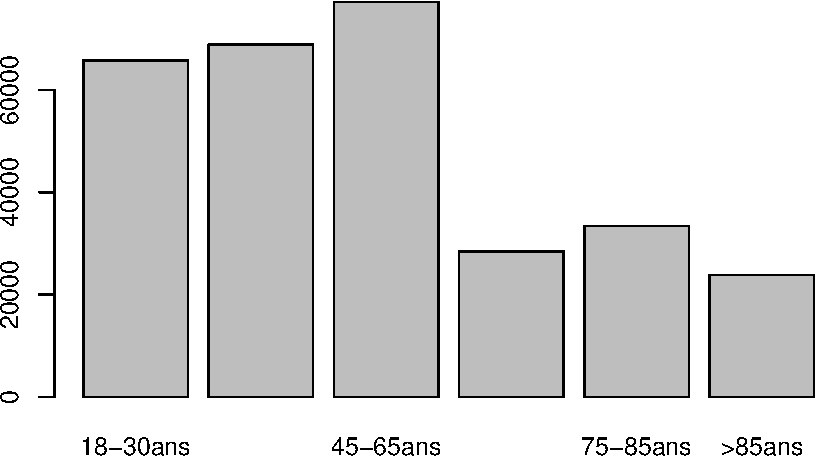
\includegraphics{age_files/figure-latex/tranches_age_als-1.pdf}
\end{figure}

\subsection{Comparaison des sex-ratio (RPU -
pop.Alsacienne)}\label{comparaison-des-sex-ratio-rpu---pop.alsacienne}

\begin{Shaded}
\begin{Highlighting}[]
\KeywordTok{plot}\NormalTok{(sr_age_rpu, }\DataTypeTok{type=}\StringTok{"l"}\NormalTok{, }\DataTypeTok{main=}\StringTok{"Evolution du sexe-ratio en fonction de l'âge"}\NormalTok{, }\DataTypeTok{ylab=}\StringTok{"Sexe-ratio"}\NormalTok{, }\DataTypeTok{xlab=}\StringTok{"Age (années)"}\NormalTok{, }\DataTypeTok{lwd=}\DecValTok{3}\NormalTok{, }\DataTypeTok{col=}\StringTok{"red"}\NormalTok{, }\DataTypeTok{ylim =} \KeywordTok{c}\NormalTok{(}\DecValTok{0}\NormalTok{, }\FloatTok{1.5}\NormalTok{))}
\KeywordTok{abline}\NormalTok{(}\DataTypeTok{h=}\DecValTok{1}\NormalTok{, }\DataTypeTok{lty=}\DecValTok{2}\NormalTok{)}
\KeywordTok{lines}\NormalTok{(sr_age, }\DataTypeTok{col=}\StringTok{"blue"}\NormalTok{, }\DataTypeTok{lty =} \DecValTok{2}\NormalTok{, }\DataTypeTok{lwd =} \DecValTok{3}\NormalTok{) }\CommentTok{# ajout de la région}
\KeywordTok{legend}\NormalTok{(}\StringTok{"bottomleft"}\NormalTok{, }\DataTypeTok{legend=}\KeywordTok{c}\NormalTok{(}\StringTok{"RPU 2014"}\NormalTok{, }\StringTok{"Population Alsace (INSEE)"}\NormalTok{), }\DataTypeTok{col=}\KeywordTok{c}\NormalTok{(}\StringTok{"red"}\NormalTok{,}\StringTok{"blue"}\NormalTok{), }\DataTypeTok{lty=}\KeywordTok{c}\NormalTok{(}\DecValTok{1}\NormalTok{,}\DecValTok{2}\NormalTok{), }\DataTypeTok{lwd=}\DecValTok{3}\NormalTok{, }\DataTypeTok{bty=}\StringTok{"n"}\NormalTok{)}
\end{Highlighting}
\end{Shaded}

\begin{figure}[htbp]
\centering
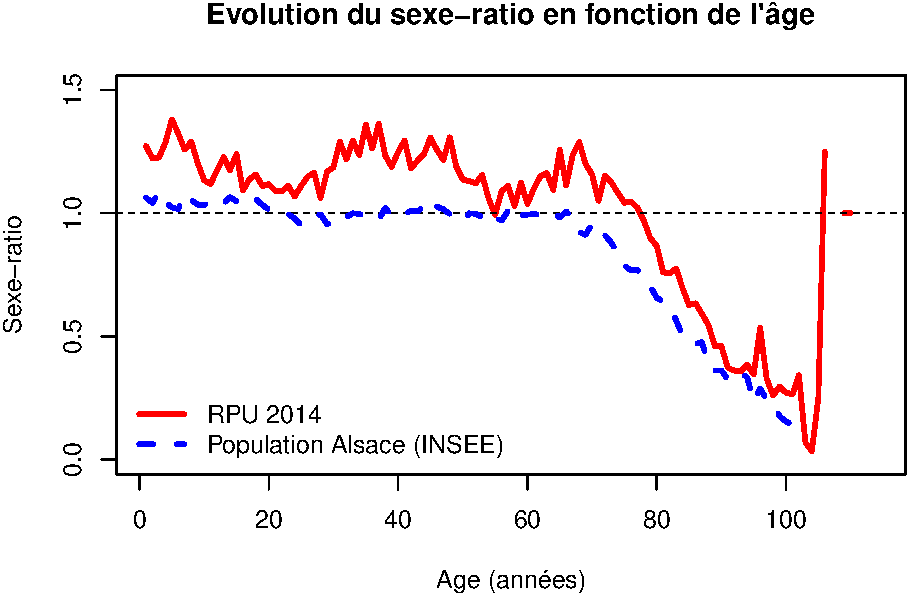
\includegraphics{age_files/figure-latex/comp_sex_ratio-1.pdf}
\end{figure}

suite

\begin{Shaded}
\begin{Highlighting}[]
\NormalTok{a <-}\StringTok{ }\KeywordTok{matrix}\NormalTok{(}\KeywordTok{c}\NormalTok{(h_rpu/N, nh_als/nAls_2014, f_rpu/N, nf_als/nAls_2014), }\DataTypeTok{nrow=}\DecValTok{2}\NormalTok{)}
\KeywordTok{barplot}\NormalTok{(a, }\DataTypeTok{beside=}\OtherTok{TRUE}\NormalTok{, }\DataTypeTok{main=}\StringTok{"Répartition des passages aux urgences 2014 par sexe"}\NormalTok{, }\DataTypeTok{ylab=}\StringTok{"%"}\NormalTok{, }\DataTypeTok{names.arg=}\KeywordTok{c}\NormalTok{(}\StringTok{"Hommes"}\NormalTok{, }\StringTok{"Femmes"}\NormalTok{))}
\KeywordTok{legend}\NormalTok{(}\DecValTok{3}\NormalTok{,}\FloatTok{0.03}\NormalTok{, }\DataTypeTok{legend=}\KeywordTok{c}\NormalTok{(}\StringTok{"RPU"}\NormalTok{,}\StringTok{"Alsace"}\NormalTok{), }\DataTypeTok{col=}\KeywordTok{c}\NormalTok{(}\StringTok{"gray50"}\NormalTok{, }\StringTok{"gray90"}\NormalTok{), }\DataTypeTok{pch=}\DecValTok{15}\NormalTok{, }\DataTypeTok{horiz=}\OtherTok{TRUE}\NormalTok{, }\DataTypeTok{bty=}\StringTok{"n"}\NormalTok{)}
\end{Highlighting}
\end{Shaded}

\begin{figure}[htbp]
\centering
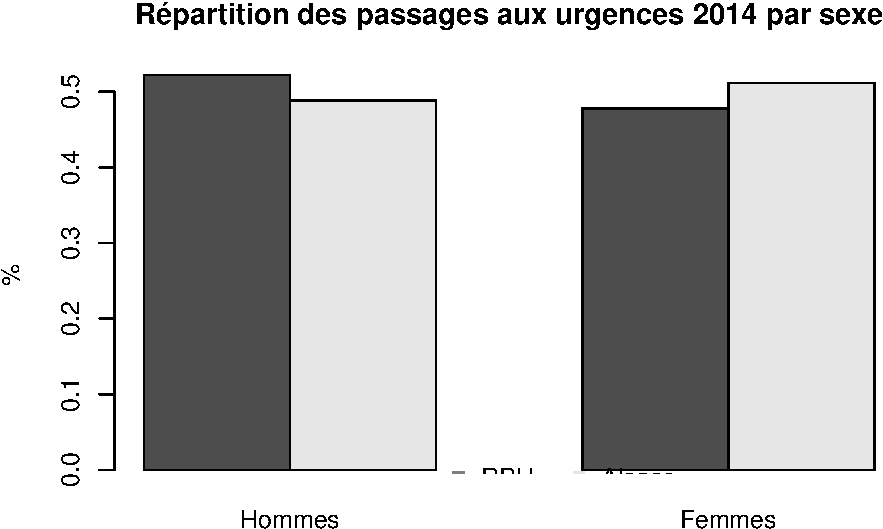
\includegraphics{age_files/figure-latex/unnamed-chunk-2-1.pdf}
\end{figure}

\paragraph{Comparaison Passages -
Population}\label{comparaison-passages---population}

On combine dans une matrice les effectifs en pourcentages par classes
d'âge (FEDORU) des passages ayant donné lieu à un RPU et ceux de la
population totale d'Alsace. Le rapport s'inverse pour la classe 85 ans
et plus.

\begin{Shaded}
\begin{Highlighting}[]
\NormalTok{a <-}\StringTok{ }\KeywordTok{rbind}\NormalTok{(adultes_als *}\StringTok{ }\DecValTok{100} \NormalTok{/}\StringTok{ }\NormalTok{n67_2014, adultes_rpu *}\StringTok{ }\DecValTok{100} \NormalTok{/}\StringTok{ }\NormalTok{N)}
\KeywordTok{rownames}\NormalTok{(a) <-}\StringTok{ }\KeywordTok{c}\NormalTok{(}\StringTok{"Alsace"}\NormalTok{,}\StringTok{"RPU"}\NormalTok{)}
\NormalTok{a}
\end{Highlighting}
\end{Shaded}

\begin{verbatim}
##        18-30ans 30-45ans 45-65ans 65-75ans 75-85ans >85ans
## Alsace       26       34       46     13.7       10    4.3
## RPU          16       17       19      6.8        8    5.7
\end{verbatim}

\begin{Shaded}
\begin{Highlighting}[]
\KeywordTok{barplot}\NormalTok{(a, }\DataTypeTok{beside=}\OtherTok{TRUE}\NormalTok{, }\DataTypeTok{main=}\StringTok{"Comparaison RPU et population adulte Alsacienne"}\NormalTok{, }\DataTypeTok{ylab=}\StringTok{"% de la population"}\NormalTok{, }\DataTypeTok{cex.names=}\FloatTok{0.8}\NormalTok{)}
\KeywordTok{legend}\NormalTok{(}\StringTok{"topright"}\NormalTok{, }\DataTypeTok{legend=}\KeywordTok{c}\NormalTok{(}\StringTok{"Alsace"}\NormalTok{,}\StringTok{"RPU"}\NormalTok{), }\DataTypeTok{pch=}\DecValTok{15}\NormalTok{, }\DataTypeTok{bty=}\StringTok{"n"}\NormalTok{, }\DataTypeTok{col=}\KeywordTok{c}\NormalTok{(}\StringTok{"black"}\NormalTok{,}\StringTok{"gray"}\NormalTok{))}
\end{Highlighting}
\end{Shaded}

\begin{figure}[htbp]
\centering
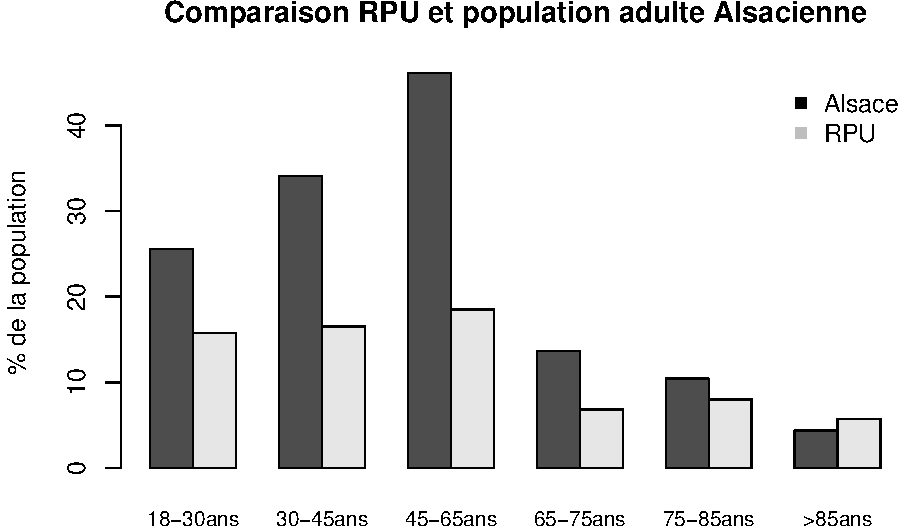
\includegraphics{age_files/figure-latex/rpu_pop-1.pdf}
\end{figure}

\section{Taux de passage}\label{taux-de-passage}

Le taux de passage: nombre de RPU / population estimée.

Pour l'ensemble de l'Alsace:

\begin{Shaded}
\begin{Highlighting}[]
\NormalTok{tx_passage <-}\StringTok{ }\NormalTok{N /}\StringTok{ }\NormalTok{nAls_2014}
\NormalTok{tx_passage}
\end{Highlighting}
\end{Shaded}

\begin{verbatim}
## [1] 0.22
\end{verbatim}

Taux de passage par tranches d'age:

\begin{Shaded}
\begin{Highlighting}[]
\NormalTok{tx_passage_age <-}\StringTok{ }\KeywordTok{as.numeric}\NormalTok{(adultes_rpu) /}\StringTok{ }\NormalTok{adultes_als}
\NormalTok{tx_passage_age}
\end{Highlighting}
\end{Shaded}

\begin{verbatim}
## 18-30ans 30-45ans 45-65ans 65-75ans 75-85ans   >85ans 
##     0.23     0.18     0.15     0.19     0.29     0.50
\end{verbatim}

A calculer également par SU.

\end{document}
